\chapter{Verification of Two Tension Cases from Allen and Wells (2014)} \label{chap:app-verification-allen-wells}

\section{Extracting Normalized Results from the TASC Database}

The TASC source code \citep{tasc} includes a MATLAB MAT file \path{interp_solution_database.mat}.
The data contained in this file is the closest representation of the original FEA solutions.
The file contains a variable \verb|result| that is a four-dimensional array indexed by \(\frac{a}{t}\), \(\frac{a}{c}\), \(n\), and \(\frac{E}{\Sys}\).
Each element in the array is a structure containing one field \verb|fea|, and that field contains other fields of the FEA results for that specific case including \verb|St_far| for a vector of far-field stress for each load step, \verb|Jtotal_Avg| for a two-dimensional array of \J values for each angle and load step, and \verb|CMOD| for a vector of CMOD values for each load step.
\Cref{fig:tasc_fea_inputs} shows the plot of far-field stress versus CMOD for \(\frac{E}{\Sys} = 100\) and \(\frac{E}{\Sys} = 200\), which is a subset of the results from \Cref{fig:modulus-gap}(a).
\begin{figure}[bp]
\centering
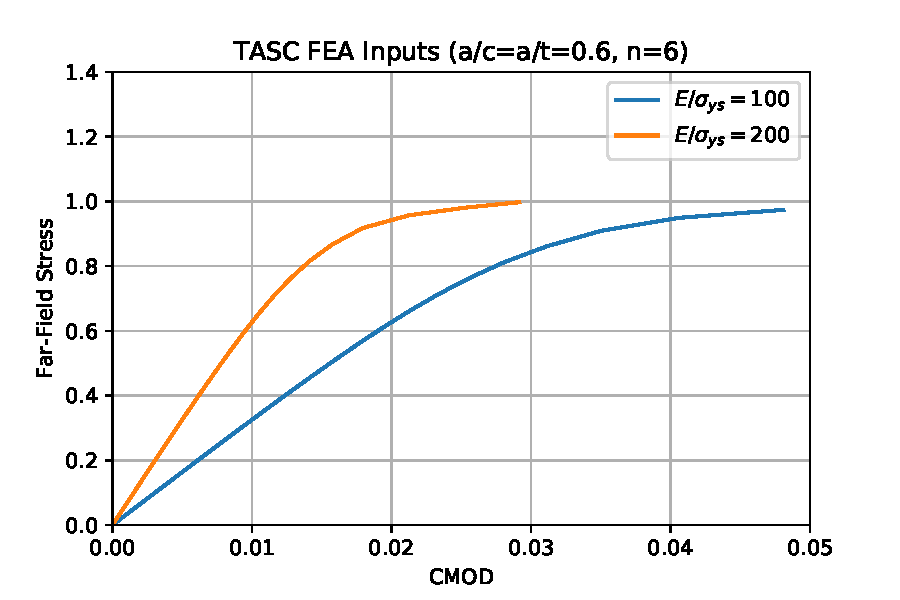
\includegraphics[width=0.8\columnwidth]{tasc-inputs}
\caption{\label{fig:tasc_fea_inputs} Raw FEA results used in TASC}
\end{figure}
\Cref{fig:tasc_interp_outputs} shows the equivalent results from the TASC program itself, after the truncation and linear extrapolation process described in \citeauthor[p.~180]{allenwells2014} has completed.
It also shows TASC's interpolated estimate for the stress-CMOD relationship for \(\frac{E}{\Sys} = 150\).
\begin{figure}[tbp]
\centering
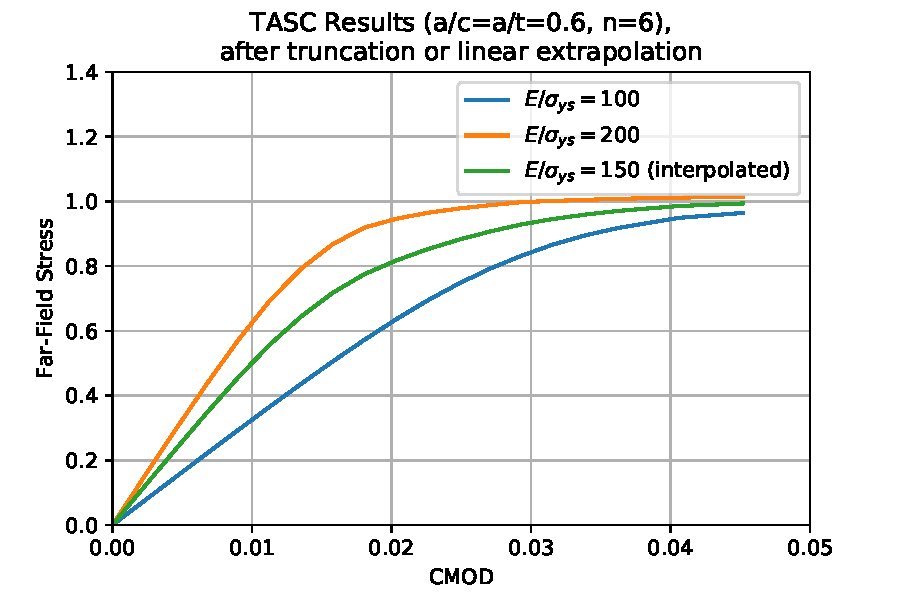
\includegraphics[width=0.8\columnwidth]{tasc-results}
\caption{\label{fig:tasc_interp_outputs} Interpolated FEA results displayed by TASC}
\end{figure}

\section{Reconstructing Model Geometry in FEACrack}

\citeauthor[p.~178]{allenwells2014} describe the cracked plate geometry and the number of nodes, elements, and nodes along the crack front for all cases. All models use a plate thickness of 1.0.
For \(\frac{a}{c}=0.6\), \(\frac{a}{t}=0.6\), the model parameters include
\begin{align*}
2c &= 2 & \text{Total nodes} &= 43,330\\
W &= 10 & \text{Total elements} &= 9,324 \\
L &= 20 & \text{Crack front nodes} &= 91
\end{align*}
and the models are built using quarter-symmetry, 20-node isoparametric elements, and ten rings of elements around the crack front for calculating the \J integral.

To recreate the model geometry in FEACrack, the following values were used in each dialog:

\begin{description}
\item[Geometry configuration] structural shape: flat plate, weld: no weld, unchecked unique materials on both sides of crack
\item[Crack configuration] crack location and orientation: build mesh in \(-Z\) direction, perpendicular to stress -- center of plate, the model is 1/4 symmetric
\item[Crack configuration, mesh options, crack mesh] use 20-node brick elements, maintain through-thickness refinement, multiple mesh stretch multipliers, 1 crack block, \(X\) and \(Y\) multipliers = 1, \(Z\) multiplier = 2, 10 rings in crack tube, 3x refinement along full crack front, auto mesh block type
\item[Crack configuration, mesh options, crack analysis] use linear kinematic element formulation (small strain), create crack mesh with no small radius keyhole (collapsed elements at the crack front)
\end{description}

A standard tension model (\path{tens.elt}) was saved with those parameters.
Early iterations of these models required manually adjusting geometry values in the FEACrack graphical user interface.
Later iterations took advantage of FEACrack accepting command-line arguments to create new models and meshes with arbitrary dimensions for both the plate and the crack.
This feature was exploited to create a plate with the correct geometry, and will be used for future models.
A copy of the standard tension model was saved under the name \path{tens_ac0.60_at0.60_L10.00_W05.00.elt}, and the FEACrack executable was run as
\begin{Verbatim}[frame=single]
feacrack.exe tens_ac0.60_at0.60_L10.00_W05.00.elt
  /ModelWidth 5.0 /ModelThickness 1.0 /ModelLength 10.0
  /CrackLength 2.0 /CrackDepth 0.6 /BuildMesh
\end{Verbatim}
to update the .elt file with the specified parameters, and build a WARP3D mesh file (\path{tens_ac0.60_at0.60_L10.00_W05.00_wrp.inp}).
The resulting mesh from these settings contains 43,330 nodes and 9,324 elements, identical to the values in the original study.
An overall view of the mesh is shown in \Cref{fig:mesh-iso}, and the crack front details are shown in \Cref{fig:mesh-front}.
It can be seen that there are 15 elements distributed along the crack perimeter, and each of those elements is refined to three elements closer to the crack front, resulting in 45 elements along the crack front.
Each element has nodes on its corners and the midpoints of its edges, resulting in 91 nodes along the crack front.
\begin{figure}[tbp]
\centering
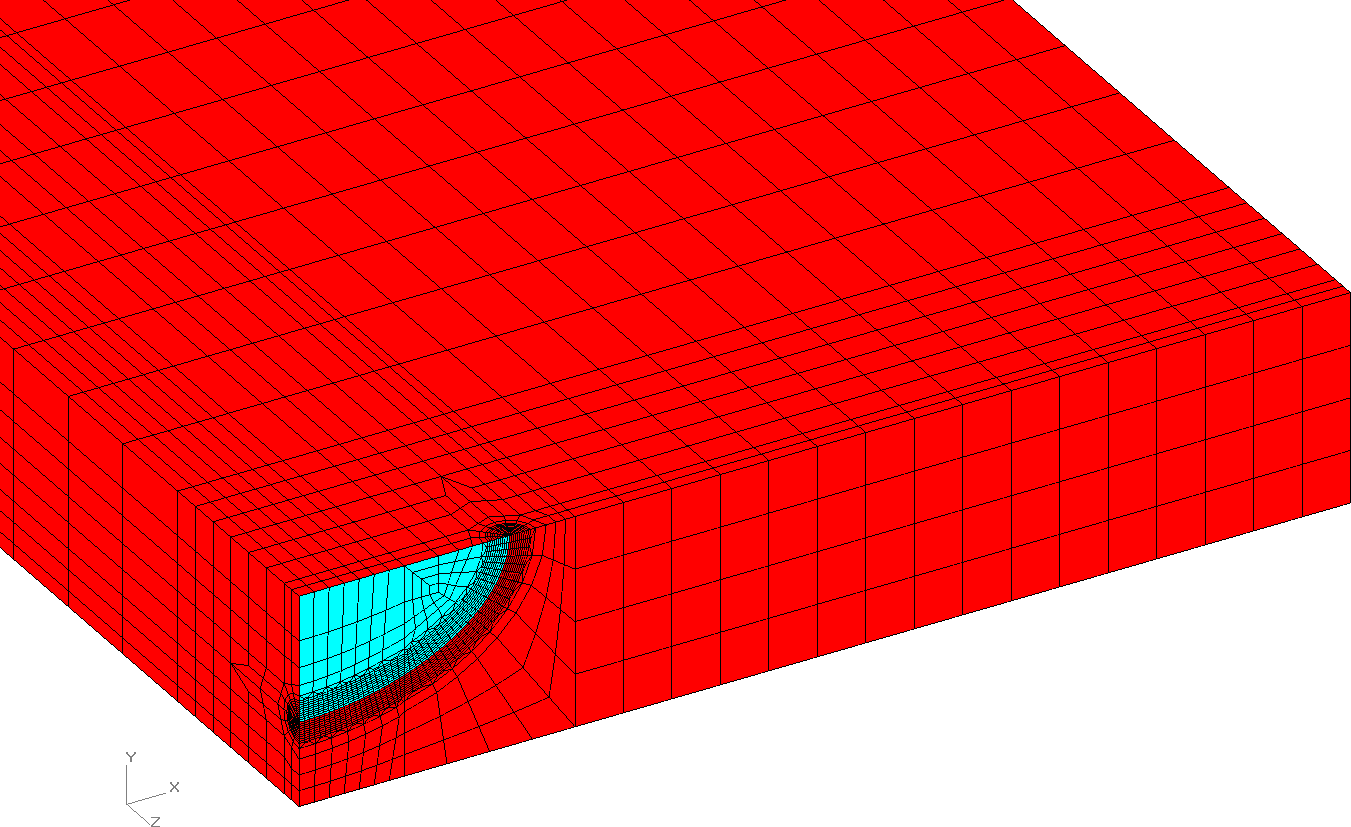
\includegraphics[width=0.8\columnwidth]{mesh-iso}
\caption{\label{fig:mesh-iso} Isometric view of overall mesh}
\end{figure}
\begin{figure}[tbp]
\centering
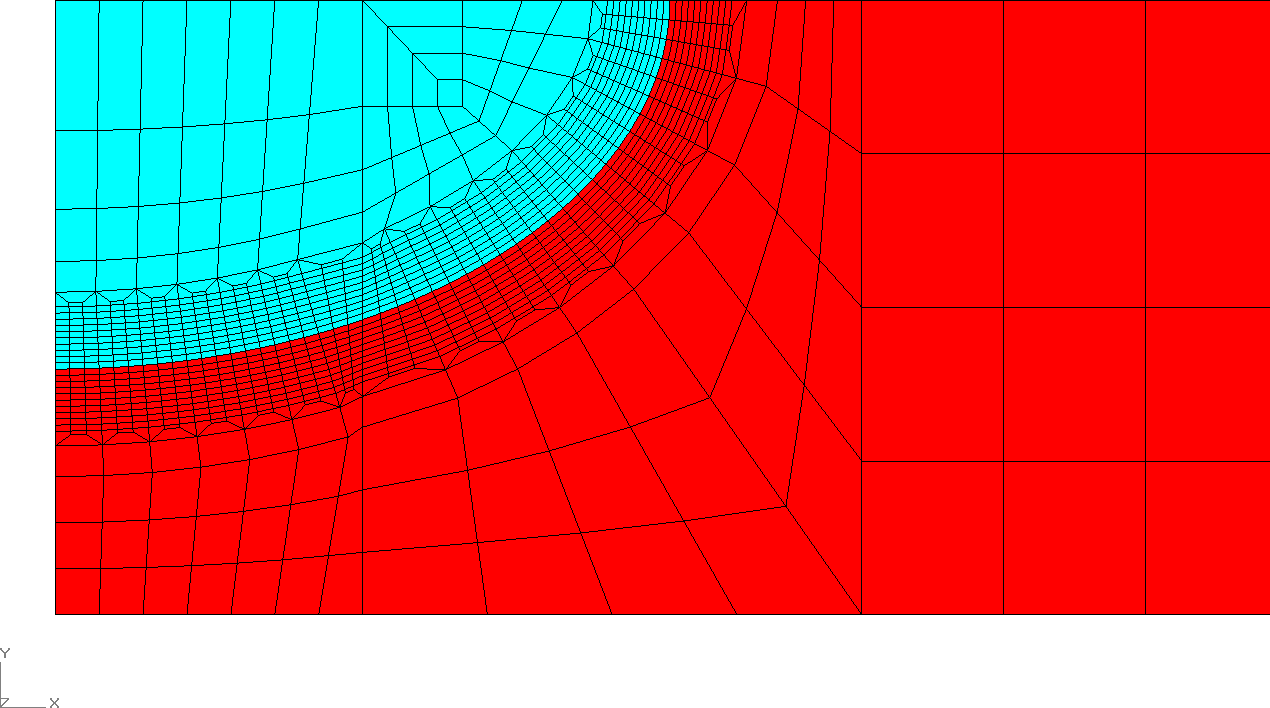
\includegraphics[width=0.8\columnwidth]{mesh-front}
\caption{\label{fig:mesh-front} Detailed view of crack front}
\end{figure}

\section{Reconstructing Material Parameters in FEACrack}

FEACrack supports the linear plus power law (LPPL) material model used in WARP3D, but \citeauthor{allenwells2014} created equivalent stress-strain curves so that their models could be analyzed in programs other than WARP3D.
All cases in their models used \(\Sys=1\) and \(\nu=0.3\), and varied \(E\) values as necessary.
For the LPPL model, the stress strain curve is defined piecewise as
\begin{align*}
\frac{\epsilon}{\epsilon_\text{ys}} &= 
\begin{cases}
\begin{aligned} % https://tex.stackexchange.com/a/385172
\hspace*{0.77em} \dfrac{\sigma}{\Sys} &,\enskip \epsilon \leq \epsilon_\text{ys} \\
\left(\dfrac{\sigma}{\Sys}\right)^{n} &,\enskip \epsilon > \epsilon_\text{ys}
\end{aligned}
\end{cases}
\end{align*}
where \(\epsilon_\text{ys} = \frac{\Sys}{E}\).
To provide a smooth transition across the part of the stress-strain curve with the highest curvature, the plastic strain values are incremented by 0.001 for 8 segments, by 0.005 for 4 segments, and by 0.010 for 7 segments.
\Cref{fig:lppl} shows a set of LPPL stress-strain curves for \(n=6\), which can be compared to Figure~2 of \citeauthor[p.~177]{allenwells2014}.
\begin{figure}[tbp]
\centering
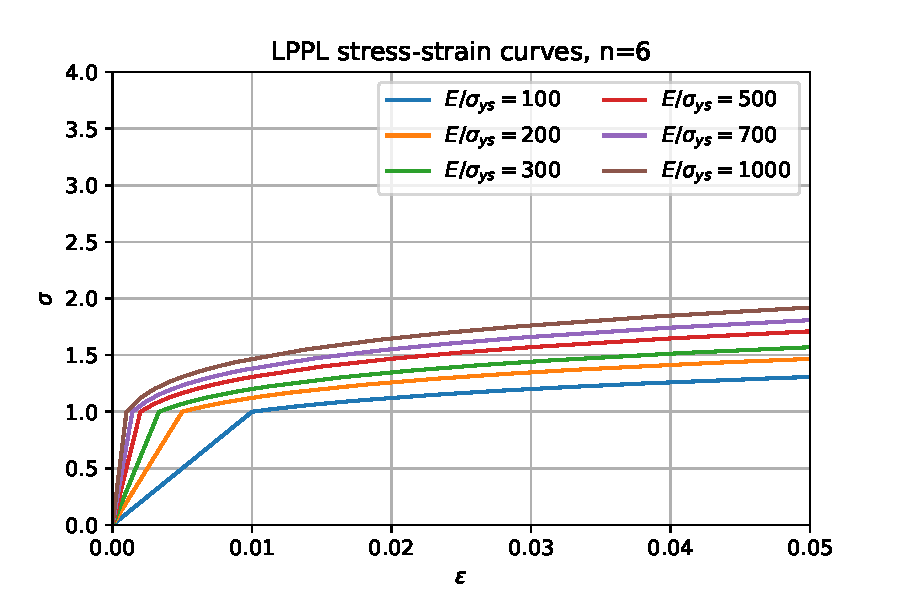
\includegraphics[width=0.8\columnwidth]{lppl}
\caption{\label{fig:lppl} Set of LPPL stress-strain curves}
\end{figure}
Early versions of these models required pasting in LPPL data and adjusting elastic properties in the FEACrack Plate Material Properties dialog window.
Later iterations used a Python function to modify the stress-strain curve data and the elastic properties in the WARP3D input file, and to also modify the corresponding comments describing the material properties.

\section{Applying Appropriate Boundary Conditions in FEACrack}

\citeauthor[p.~178]{allenwells2014} noted the need to adjust displacement boundary conditions to deform the model far into the plastic regime, but not so far as to fail to converge on later load steps.
As the required deformation levels are affected by material strength, \J values, and model dimensions, they defined a dimensionless deformation parameter around the crack front
\begin{align*}
M &= \frac{r_\phi \Sys}{\J}
\end{align*}
where \(r_\phi\) is a characteristic length of a line normal to the crack front connecting the cracked surface to the opposite surface at a given angle \(\phi\).
One characteristic length \(r_{\phi a}\) correlates to the crack length, and the other characteristic length \(r_{\phi b}\) correlates to the length of the uncracked ligament.
Displacement values were modified until \(M\) values at \(\phi = \) \SI{30}{\degree} or \(\phi = \) \SI{90}{\degree} were around \(M \approx 20 \) or lower.
Early verification cases used remote displacement values extracted from the TASC solution database as given in \Cref{tab:displacement_values}.
\begin{table}[pb]
\caption{\label{tab:displacement_values} Applied displacement values for verification models}
\centering
\begin{tabular}{S[table-format=3.0] S[table-format=1.4] S *2{S[table-format=1.4]}} \toprule
{\(\frac{E}{\Sys}\)} & {Displacement} & {\(\phi\)} & {\(M\) using \(r_{\phi a}\)} & {\(M\) using \(r_{\phi b}\)} \\ \midrule
100 & 0.1028 & \SI{30}{\degree} & 15.9833 & 36.4241 \\
    &        & \SI{90}{\degree} & 22.6234 & 15.0822 \\
200 & 0.0550 & \SI{30}{\degree} & 24.7288 & 56.3542 \\
    &        & \SI{90}{\degree} & 34.9604 & 23.3069 \\
\bottomrule
\end{tabular}
\end{table}
(0.1028 inches for \(\frac{E}{\Sys} = 100\), and 0.0550 inches for \(\frac{E}{\Sys} = 200\)).
Later verification cases employed a Python function using the secant method to adjust the boundary condition in the WARP3D input file until the smallest of the \(M\) values was in the range of \([20, 25]\).
The Python program sets the initial boundary condition to a value corresponding to a net section stress of \(0.9\Sys\), and uses an objective function of the form:
\begin{align*}
\text{Error} &= 
\begin{cases}
\begin{aligned} % https://tex.stackexchange.com/a/385172
0 &,\enskip 20 \leq M \leq 25 \\
|M-22.5| &,\enskip \text{otherwise}
\end{aligned}
\end{cases}
\end{align*}
to drive the boundary condition to the correct level.

\section{Solving Models in WARP3D}

Early iterations of these models used FEACrack's ``Build Mesh'' button was used to write out a WARP3D input file containing the nodes, elements, material properties, and boundary conditions for the given cracked plate.
The \(\frac{E}{\Sys}=100\) model with 30 load steps and an applied displacement of 0.1028~inches was solved on two different computers running WARP3D.
In both cases, WARP3D was run with a command of the form {\ttfamily warp3d < file.inp > file.out}.
A Windows 10 virtual machine with 2 2.6~GHz i5-4288U processor cores and 8~GB of memory solved the model in 21.6 minutes, and
a Linux server in the TTU HPC with 28 2.4~GHz Xeon E5-2680v4 processor cores and 128~GB of memory solved the model in 2.2 minutes.
In both cases, WARP3D wrote a plain-text output file including \J values for each of the 91 crack front positions at all load steps, and also wrote a binary packet file with more detailed results including nodal displacements and reaction forces for all nodes at all load steps.

Later iterations used a Python program to automate these tasks.
When the secant method was used to modify the boundary condition, each iteration of the secant method took roughly 90 seconds to solve.
This method was slightly faster as the applied boundary condition was smaller than 0.1028 inches, and the solver spent less time in the plastic regime.

\section{Analyzing WARP3D Results}

WARP3D binary packet files (\path|*_wrp.bpf|) can be analyzed with three different methods:
\begin{enumerate}
\item Reading the files into FEACrack interactively,
\item Using the FEACrack \verb|/PostProcess|, \verb|/BuildMesh|, and \verb|/RunFEA| parameters,
\item Using the \path{packet_reader} FORTRAN program to convert the binary packets into a text form.
\end{enumerate}
The \path{packet_reader} FORTRAN source code was compiled on the TTU HPC and used to first export the reaction forces for all nodes at all load steps, and then to export all the displacements for all nodes at all load steps.
A Python program was written to extract selected results from the reaction and displacement files:
\begin{enumerate}
\item reaction forces in the \(z\) direction of all nodes contained in the \(z=0\) plane (these nodes were identified by examining the nodal coordinates list in the WARP3D input file),
\item \(z\) direction displacement of the node at \((x, y, z) = (0, 0, 0)\), identical to half of the CMOD on an experiment due to model symmetry.
\end{enumerate}
The \(z=0\) plane contains nodes inside the crack, where reaction forces should be zero, and also nodes along the symmetry plane, comprising all the reaction to maintain static equilibrium when displacements are applied at the remote end.

The reaction force and CMOD values for the \(\frac{E}{\Sys} = 100\) model were imported into Python.
The reaction force sign was changed, since all the reaction force results were negative, and then divided by the plate nominal area (\(W=5\), \(t=1\)) to calculate a remote stress.
The displacement results were doubled to match the definition of CMOD.
The transformed remote stress and CMOD data were plotted over the existing results, and the results can be seen in \Cref{fig:e100_verification,fig:e100_200_verification}.
In both models, the new results match the corresponding original models.
\begin{figure}[tbp]
\centering
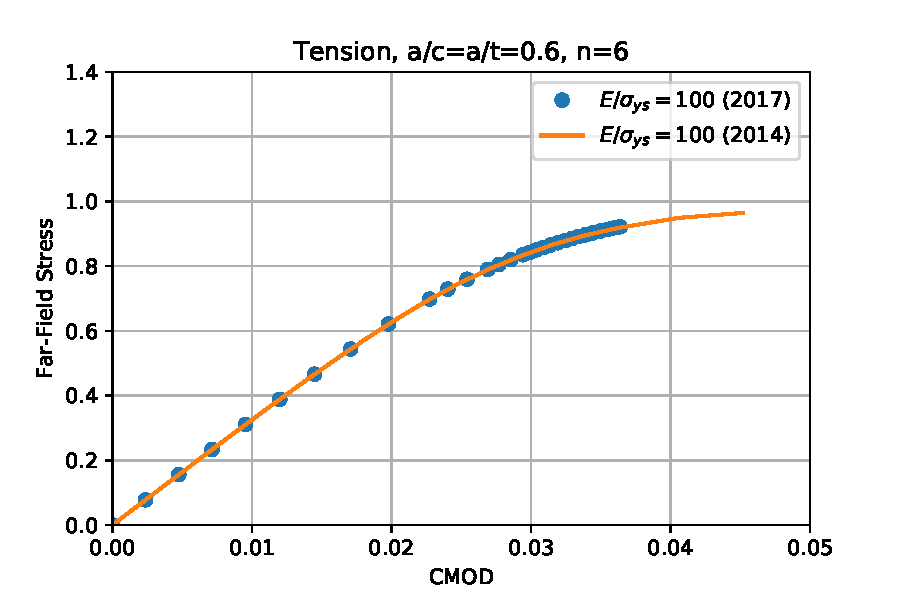
\includegraphics[width=0.8\columnwidth]{e100_verification}
\caption{\label{fig:e100_verification} Verification of stress and CMOD relationship for first model}
\end{figure}
\begin{figure}[tbp]
\centering
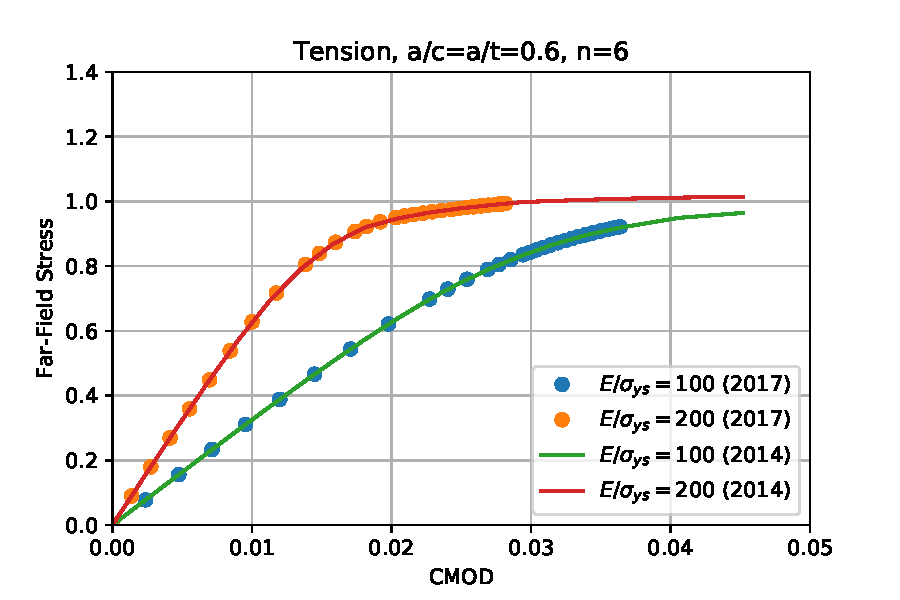
\includegraphics[width=0.8\columnwidth]{e100_200_verification}
\caption{\label{fig:e100_200_verification} Verification of stress and CMOD relationship for second model}
\end{figure}
